\documentclass[a4paper, 12pt]{article}%тип документа

%отступы
\usepackage[left=2cm,right=2cm,top=2cm,bottom=3cm,bindingoffset=0cm]{geometry}

%Русский язык
\usepackage[T2A]{fontenc} %кодировка
\usepackage[utf8]{inputenc} %кодировка исходного кода
\usepackage[english,russian]{babel} %локализация и переносы

%Вставка картинок
\usepackage{wrapfig}
\usepackage{graphicx}
\graphicspath{{pictures/}}
\DeclareGraphicsExtensions{.pdf,.png,.jpg}

%оглавление
\usepackage{titlesec}
\titlespacing{\chapter}{0pt}{-30pt}{12pt}
\titlespacing{\section}{\parindent}{5mm}{5mm}
\titlespacing{\subsection}{\parindent}{5mm}{5mm}
\usepackage{setspace}

%Графики
\usepackage{multirow}
\usepackage{pgfplots}
\pgfplotsset{compat=1.9}

%Математика
\usepackage{amsmath, amsfonts, amssymb, amsthm, mathtools}

%Стиль страницы
\usepackage{fancyhdr}
\pagestyle{fancy}

\begin{document}

\begin{titlepage}

\begin{center}
%\vspace*{1cm}
\large\textbf{Московский Физико-Технический Институт}\\
\large\textbf{(государственный университет)}
\vfill
\line(1,0){430}\\[1mm]
\huge\textbf{Работа 4.3.4.}\\
\line(1,0){430}\\[1mm]
\vfill
\large Сибгатуллин Булат, ФРКТ\\
\end{center}

\end{titlepage}
\fancyhead[L] {Работа 4.3.4.}
\noindent \textbf{Цель работы:} \\
\indent Определить размеры щели, определить периоды сеток; исследовать изображение щели.\\
\noindent \textbf{В работе используются:} \\
\indent Гелий-неоновый лазер, кассета с набором сеток разного периода, щель с микрометрическим винтом, линзы, экран, линейка.

\section*{Теоретическая часть}
Рассмотрим дифракцию плоской монохроматической волны на синусоидальной амплитудной решётке. Пусть решётка с периодом d расположена в $t = 0$, а её штрихи ориентированы вдоль $OY$. Тогда функция пропускания:
\[
	t(x) = \beta  + \alpha cos(ux) = \beta + \alpha \frac{e^{iux} + e^{-iux}}{2},
\]
где $\alpha, \beta = const, u = \frac{2 \pi}{d}$.

Если на решётку падает плоская моно волна вдоль $OZ$:
\[
	E(\vec r, t) = E_0 e^{-i(\omega t - kz)},
\]
то на выходе получим три плоских волны:
\[
	E_1 = \beta E_0 e^{-i (\omega t - kz)};
\]
\[
	E_2 = \frac{\alpha}{2} E_0 e^{-i (\omega t - ux - \sqrt{k^2 - u^2}z)};
\]
\[
	E_3 = \frac{\alpha}{2} E_0 e^{-i (\omega t + ux - \sqrt{k^2 - u^2}z)},
\]
где $\omega$ "--- круговая частота, $k = \frac{2 \pi}{\lambda}$ "--- волновой вектор, $E_0$ "--- амплитуда.
Каждая из этих трёх волн фокусируется линзой в точку в задней фокальной плоскости. Волна $E_1$ (вдоль $OZ$) фокусируется в начало координат, волны $E_2$ И $E_3$ (распространяются в направлении $\sin \theta = \pm \frac{u}{k}$) фокусируются в точке $x_1 = \pm \frac{Fu}{k} = \pm {F \lambda}{d}$, где $F$ "--- фокусное расстояние линзы.

Теорема Фурье в комплексной форме:
\[
	t(x) = \sum_{n = - \infty}^\infty C_n e^{inux},
\]
сумма бесконечного множества канонических составляющих, имеющие кратные частоты.
Картина, наблюдаемая в фурье-плоскости, представляет собой эквидистантный набор точек с координатами и амплитудами, пропорциональными $C_n$:
\[
	x_n = \frac{Fu}{k} = \frac{F \lambda}{d}n.
\]
При освещении транспаранта плоской моно волной картина, наблюдаемая в задней фокальной плоскости линзы, установленной за транспарантом, представляет собой фурье-образ функции пропускания транспаранта.
Для того, чтобы найти фурье-образ функции пропускания, достаточно определить только пространственные частоты и соотношение между амплитудами плоских волн на выходе. Для амплитудной синусоидальной решётки получаем три плоских волны с частотами $0, +u, -u$ и амплитудами, пропорциональными $\beta, \frac{\alpha}{2}, \frac{\alpha}{2}$.
\begin{figure}[h!]
	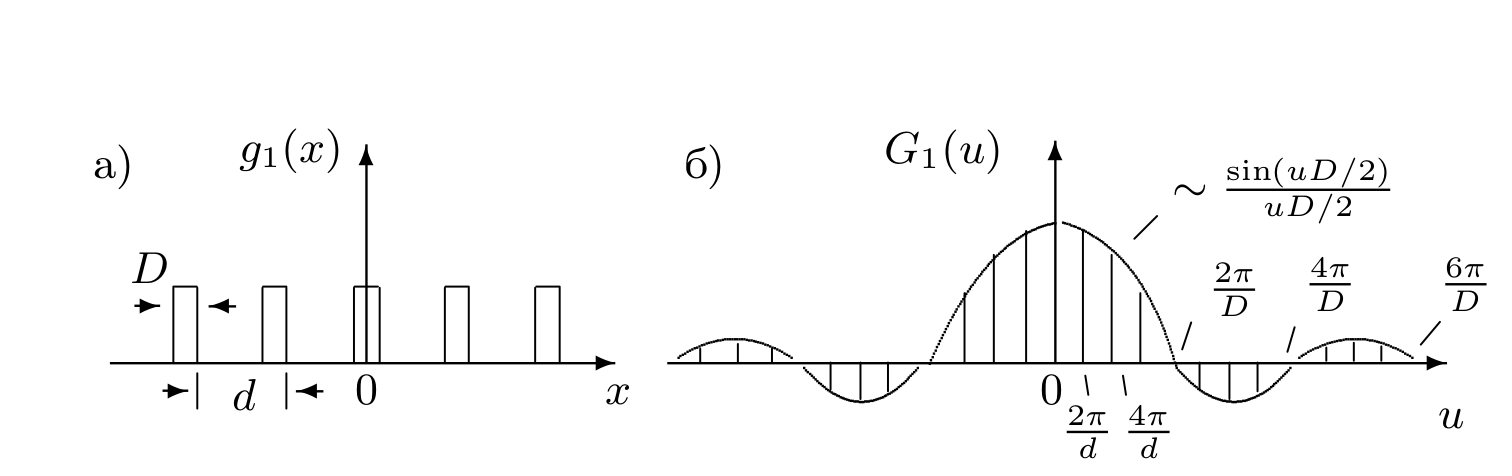
\includegraphics[width = 1.0\linewidth]{images/5.png}
	\caption{а) функция пропускания дифракционной решётки (последовательности прозрачных и непрозрачных полос);\\
б) $G_1 (u)$ "--- спектр функции пропускания дифракционной решётки}
\end{figure}	
Пространственное преобразование Фурье может осуществляться и в свободном пространстве при наблюдении дифракции Фраунгофера.
Если размеры дифракционной решётки неограничены, то дифракционные максимумы бесконечно узки. Чем меньше размер решётки (полное число щелей), тем шире каждый отдельный максимум.

Направление на главные максимумы $\theta_n = \frac{u n}{k} = \frac{\lambda n}{d}$ ($N$ "--- целое число) определяется приодом решётки d, а распределение амплитуд в спектре "--- фурье-образом функции пропускания отдельного штриха:
\[
g_2 (x) = \begin{cases} 1, & - \frac{D}{2} \leq x \leq \frac{D}{2} \\
						0, & - \frac{D}{2} > x > \frac{D}{2}
\end{cases}
\]
Вследсвие непереодичности $g_2(x)$, её фурье-образ представлятся непрерывным множеством точек и определяется интегралльным преобразованием Фурье:
\[
g(x) = \frac{1}{2 \pi} \int_{-\infty}^{+\infty} G(u) e^{iux} du,
\]
\[
G(u) = \int_{-\infty}^{+\infty} g(x) e^{-iux}dx.
\]
В таком виде $g(x)$ и $G(u)$ представляют собой пару преобразований Фурье: $G(u)$ "--- спектр или фурье-образ функци $g(x)$.
\[
	G_2 (u) = \int_{-\infty}^{+\infty} g_2 (x) e^{-iux} dx  = \int_{-D/2}^{+D/2} e^{-iux} dx = D \frac{\sin \frac{uD}{2}}{\frac{uD}{2}}.
\]
Введём понятие протяженности функции пропускания транспоранта ($\Delta x$) и ширины её спектра ($\Delta u$), тогда соотношение неопределённости принимает вид:
\[
	\Delta x \cdot \Delta u = \frac{2 \pi}{D} \cdot D = 2 \pi.
\]
Размер же малого объекта можно рассчитать, увеличив его изображение с помощью линзы.

\textbf{Метод Аббе}
Рассмотрим схему образования изображения. Пусть предмет расположен от линзы на большем расстоянии, чем фокусное, тогда существует сопряжённая предметной плоскости плоскость, где образуется изображение. Аббе предложил рассматривать схему прохождения в два этапа: сначала рассматривается первичное изображение (спектр в задней фокальной плоскости), затем это изображение рассматривается как источник волн, создающий изображение в другой плоскости (вторичное изображение). Этот подход опирается на принцип Гюйгенса-Френеля, согласно которому любой участок волнового фронта можно рассматривать как источник излучения. Под словами <<линза дважды осуществляет преобразование Фурье>> подразумевается следующее: сначала в задней фокальной плоскости линзы получается световое поле, соответствующее фурье-образу функции пропускания предмета (с точностью до фазы), а затем на промежутке между фокальной плоскостью и плоскостью изображения осуществляется обратное преобразование Фурье, в результате чего восстанавливается изображение предмета.

\textbf{Определение ширины щели с помощью линзы}
\begin{figure}[h!]
	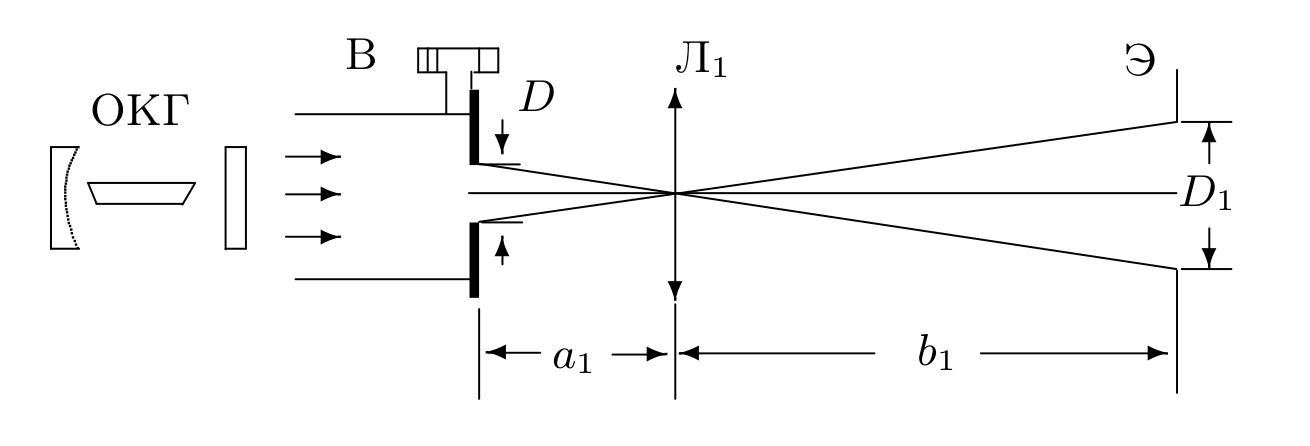
\includegraphics[width = 1.0\linewidth]{images/1.png}
	\caption{Схема для определения ширины щели с помощью линзы}
\end{figure}


\end{document}